\documentclass[a4paper,dvipdfmx,11pt,reqno]{amsart}
\usepackage{amsmath,amsthm,amssymb,mathrsfs,stmaryrd}
\usepackage{bm}
% \usepackage[bbgreekl]{mathbbol}
\usepackage{url}
\usepackage{color}
\usepackage{eucal}
\usepackage{slashed}
\usepackage{physics}
\usepackage{graphicx}
\usepackage{tikz}
\usepackage{tikz-cd}
\usepackage{tikz-3dplot}
\usetikzlibrary{intersections, calc, arrows, arrows.meta, shadows}
\usepackage[utf8]{inputenc} % for special characters
\usepackage[T1]{fontenc}
\usepackage[backend=biber,style=alphabetic,hyperref=true]{biblatex} % for bib-latex
\addbibresource{references_algebraic_k_theory.bib}
\usepackage{geometry} % margin settings
\geometry{margin=1.0in}
\usepackage{enumitem} % item style
\setlist[enumerate]{itemsep=2pt,parsep=2pt,before={\parskip=2pt}}
\setlist[description]{style=standard}
\usepackage[colorlinks=true,hyperindex, linkcolor=magenta, pagebackref=false, citecolor=cyan,pdfpagelabels]{hyperref} % link colors
\usepackage{cleveref}

\renewcommand{\baselinestretch}{1.1} % change the space between lines

\allowdisplaybreaks % allow page breaks in equations

% math definitions
\DeclareMathOperator{\Ob}{Ob}
\DeclareMathOperator{\Hom}{Hom}
\DeclareMathOperator{\Map}{Map}
\DeclareMathOperator{\Nat}{Nat}
\DeclareMathOperator{\myop}{op}
\DeclareMathOperator{\id}{id}
\DeclareMathOperator{\fib}{fib}
\DeclareMathOperator{\cofib}{cofib}
\renewcommand{\mid}{\mathrm{mid}}
\DeclareMathOperator{\const}{const}
\DeclareMathOperator*{\colim}{colim}
\renewcommand{\ev}{\mathrm{ev}}
\DeclareMathOperator{\h}{h}
\DeclareMathOperator{\N}{N}
\DeclareMathOperator{\Fun}{Fun}

% math definitions for K-theory
\DeclareMathOperator{\Seq}{Seq}
\DeclareMathOperator{\core}{core}
\DeclareMathOperator{\asscat}{asscat}
\DeclareMathOperator{\Span}{Span}
\DeclareMathOperator{\Idem}{Idem}
\DeclareMathOperator{\Ind}{Ind}
\DeclareMathOperator{\grp}{grp}
% \newcommand{\Ksp}{\mathcal{K}^{\mathrm{sp}}}

% categories (using mathcal)
\newcommand{\A}{\mathcal{A}}
\newcommand{\B}{\mathcal{B}}
\newcommand{\C}{\mathcal{C}}
\newcommand{\D}{\mathcal{D}}
\newcommand{\E}{\mathcal{E}}
\newcommand{\F}{\mathcal{F}}
\newcommand{\G}{\mathcal{G}}
\newcommand{\I}{\mathcal{I}}
\newcommand{\J}{\mathcal{J}}
\newcommand{\K}{\mathcal{K}}
\newcommand{\V}{\mathcal{V}}
\newcommand{\W}{\mathcal{W}}
\renewcommand{\H}{\mathcal{H}}
\renewcommand{\O}{\mathcal{O}}
\renewcommand{\P}{\mathcal{P}}
\renewcommand{\S}{\mathcal{S}}

% categories (using math rm)
\newcommand{\An}{\mathrm{An}}
\newcommand{\Cat}{\mathrm{Cat}}
\newcommand{\Catlex}{\mathrm{Cat^{lex}}}
\newcommand{\Catperf}{\mathrm{Cat^{perf}}}
\newcommand{\Catst}{\mathrm{Cat^{st}}}
\newcommand{\Mon}{\mathrm{Mon}_{\mathbb{E}_{\infty}}}
\newcommand{\Grp}{\mathrm{Grp}_{\mathbb{E}_{\infty}}}
\newcommand{\Ar}{\mathrm{Ar}}
\newcommand{\TwArr}{\mathrm{TwAr^{r}}}
\newcommand{\Sp}{\mathrm{Sp}}

% math bb
\newcommand{\Einf}{\mathbb{E}_{\infty}}

% ------------------------------------------------------

\begin{document}

% theorem style (using definition style)
\newtheorem{theorem}{Theorem}[section]
\newtheorem*{definition*}{Definition}
\newtheorem*{theorem*}{Theorem}
\newtheorem*{conjecture*}{Conjecture}

\theoremstyle{definition}
\newtheorem{definition}[theorem]{Definition}
\newtheorem{conjecture}[theorem]{Conjecture}
\newtheorem{construction}[theorem]{Construction}
\newtheorem{corollary}[theorem]{Corollary}
\newtheorem{example}[theorem]{Example}
\newtheorem{lemma}[theorem]{Lemma}
\newtheorem{notation}[theorem]{Notation}
\newtheorem{proposition}[theorem]{Proposition}
\newtheorem{question}[theorem]{Question}
\newtheorem{remark}[theorem]{Remark}

% special clever-ref
\newcommand{\additivitytheorem}{\hyperref[thrm.additivity_theorem]{additivity theorem}}
\newcommand{\universalitytheorem}{\hyperref[thrm.universality_theorem]{universality theorem}}

% --------------------------------------------------

\title{The Higher Algebraic K-Theory of Stable \texorpdfstring{$\infty$}{infty}-Categories}
\author{Keima Akasaka}
\maketitle 

\begin{abstract}
  We summarize the higher algebraic K-theory of stable $\infty$-categories.
\end{abstract} 

% show depth in contents
\setcounter{tocdepth}{2}
\tableofcontents   

\section{Introduction}

This paper is a summary of the workshop on the higher algebraic K-theory held in Kyoto in September 2024.
Although we do not plan to write a detailed introduction, we are making it available to the public.
To make it easier to read, all proofs are included in Appendix (if we write).

\subsection{Notation}

From here all categories are assumed to be $\infty$-categories.
We let 
\begin{itemize}
  \item $\An$ denote the category of anima.
  \item $\Cat$ denote the category of small categories.
  \item $\Catlex$ denote the category of small categories which admit finite limits, with left exact functors.
  \item $\Catst$ denote the category of small stable categories with exact functors.
  \item $\Catperf$ denote the category of small idempotent complete stable categories with exact functors.
  \item $\Sp$ denote the category of spectra.
\end{itemize}


\section{Preliminaries}

\subsection{The Grothendieck Group} % p7

\begin{definition}
  Let $(\C,\oplus)$ be a stable category, and let $X$ and $Y$ be objects of $\C$.
  We let $[X]$ denote the connected component of $X$.
  The connected component set $\pi_0(\core\C)$, together with the operation $+$ defined by 
  \begin{align*}
    [X] + [Y] := [X \oplus Y]
  \end{align*}
  forms an ordinary monoid $(\pi_0(\core\C),+)$.
  We define the \textit{Grothendieck group} $\K_0(\C)$ of $\C$ as 
  \begin{align*}
    \K_0(\C) := (\pi_0(\core\C),+) / \sim
  \end{align*}
  where $\sim$ is the equivalence relation generated by the following relation:
  $[X]=[X']+[X'']$ whenever $X' \to X \to X''$ is a cofiber sequence in $\C$.
\end{definition}

\begin{remark}
  The connected component set $\pi_0(\core\C)$ is the set of equivalence classes of objects of $\C$.
  Moreover, the Grothendieck group $\K_0(\C)$ is actually abelian.
  \begin{enumerate}
    \item The zero object $0$ of $\C$ is a unit object $[0]$ of $\K_0(\C)$, since $X \to X \to 0$ is a cofiber sequence in $\C$ for every object $X$ of $\C$.
    \item For every object $X$ of $\C$, $[\Omega X]$ and $[\Sigma X]$ are inverse objects of $[X]$ in $\K_0(\C)$, since $\Omega X \to 0 \to X$ and $X \to 0 \to X$ are cofiber sequences in $\C$.
    \item For every objects $X$ and $Y$ of $\C$, we have $[X]+[Y]=[Y]+[X]$, since $X \to X \oplus Y \to Y$ and $Y \to X \oplus Y \to X$ are cofiber sequences in $\C$.
  \end{enumerate}
\end{remark}

\begin{remark}[Eilenberg swindle]
  Let $\C$ be a stable category with countable coproduct.
  Then the Grothendieck group $\K_0(\C)$ is trivial.
  It follows from that $X \to \oplus_{n \geq 0} X \to \oplus_{n \geq 1} X$ is a cofiber sequence in $\C$ for every object $X$ of $\C$, and that the last two terms are equivalent.
\end{remark}

\begin{remark}
  The construction $\C \mapsto \K_0(\C)$ determine a functor $\K_0 : \h\Catst \to \mathrm{Ab}$.
\end{remark}

\subsection{Arrow Categories and Twisted Arrow Categories} % p13

\begin{definition}
  Let $\C$ be a category.
  We define the \textit{arrow category} $\Ar(\C)$ of $\C$ as 
  \begin{align*}
    \Ar(\C) := \Fun([1],\C).
  \end{align*} 
\end{definition}

\begin{definition}
  Let $\C$ be a category.
  We define the \textit{twisted arrow category} $\TwArr(\C)$ of $\C$ as a right fibration classifying the mapping anima functor.
  That is, the source-target projection 
  \begin{align*}
    (s,t) : \TwArr(\C) \to \C \times \C^{\myop}
  \end{align*}
  is the right fibration classifying the mapping anima functor $\Map_{\C} : \C \times \C^{\myop} \to \An^{\myop}$.
\end{definition}

\begin{remark}
  Let $\C$ be a category.
  Let see the objects and morphisms of $\Ar(\C)$ and $\TwArr(\C)$.
  \begin{itemize}
    \item The objects of both are both morphisms in $\C$.
    \item A morphism from $f$ to $g$ in $\Ar(\C)$ is a diagram, depicted as 
    \[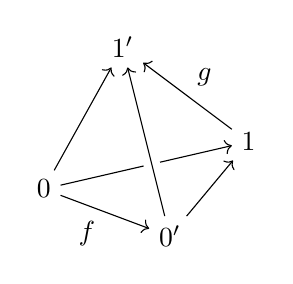
\begin{tikzpicture}[auto]
      \node (0) at (0,0) {$0$};
      \node (1) at (1.6,-0.6) {$0'$};
      \node (2) at (2.6,0.6) {$1$};
      \node (3) at (1,1.8) {$1'$};
      \draw[->] (0) -- node[swap] {$f$} (1);
      \draw[->] (0) -- node {} (2);
      \draw[->] (0) -- node {} (3);
      \draw[->] (1) -- node {} (2);
      \draw[-, line width=6pt,draw=white] (1) -- node {} (3);
      \draw[->] (1) -- node {} (3);
      \draw[->] (2) -- node[swap] {$g$} (3);
    \end{tikzpicture}\]
    \item A morphism from $f$ to $g$ in $\TwArr(\C)$ is a diagram, depicted as 
    \[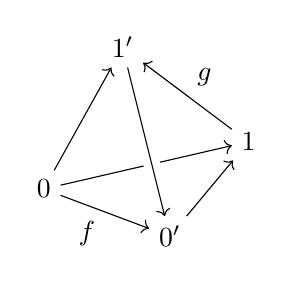
\begin{tikzpicture}[auto]
      \node (0) at (0,0) {$0$};
      \node (1) at (1.6,-0.6) {$0'$};
      \node (2) at (2.6,0.6) {$1$};
      \node (3) at (1,1.8) {$1'$};
      \draw[->] (0) -- node[swap] {$f$} (1);
      \draw[->] (0) -- node {} (2);
      \draw[->] (0) -- node {} (3);
      \draw[->] (1) -- node {} (2);
      \draw[-, line width=6pt,draw=white] (1) -- node {} (3);
      \draw[->] (3) -- node {} (1);
      \draw[->] (2) -- node[swap] {$g$} (3);
    \end{tikzpicture}\]
  \end{itemize}
\end{remark}

\begin{notation} % p49
  Let $\C$ be a stable category.
  We let $\Seq(\C)$ denote the full subcategory of $\Fun(\Delta^1 \times \Delta^1,\C)$ spanned by the bifiber sequences in $\C$.
  We have an equivalence $\Seq(\C) \simeq \Ar(\C)$, so that the category $\Seq(\C)$ is stable.
\end{notation}

\begin{notation}
  Let $\C$ be a stable category.
  We define functors from $\Seq(\C)$ to $\C$ as 
  \begin{align*}
    \fib   : \Seq(\C) \to \C &: (X \to Y \to Z) \mapsto X \\
    \mid   : \Seq(\C) \to \C &: (X \to Y \to Z) \mapsto Y \\
    \cofib : \Seq(\C) \to \C &: (X \to Y \to Z) \mapsto Z.
  \end{align*}
\end{notation}

\subsection{Verdier Sequences and Squares}

\begin{definition} % p5
  Let $\C \xrightarrow{f} \D \xrightarrow{p} \E$ be a sequence in $\Catst$.
  We will say that the sequence has \textit{vanishing composition} if the composition $pf$ is a zero object of $\Catst$.
  In this case, the functor $pf$ is equivalent to the functor $\C \to 0 \to \E$, since the full subcategory of $\Fun^{\mathrm{ex}}(\C,\E)$ spanned by the zero objects is contractible.
\end{definition}

\begin{definition} % p18
  Let $\C \xrightarrow{f} \D \xrightarrow{p} \E$ be a sequence in $\Catst$ with vanishing composition.
  We will say that this sequence is \textit{Verdier} if it is a bifiber sequence in $\Catst$.
  In this case, we will refer to the functor $f$ as the \textit{Verdier inclusion} and to the functor $p$ as the \textit{Verdier projection}.
\end{definition}

\begin{definition}
  Let $\C \xrightarrow{f} \D \xrightarrow{p} \E$ be a Verdier sequence.
  We will say that this sequence is \textit{split} if the functor $p$ admits left and right adjoint functors.
  In this case, we will refer to the functor $f$ as the \textit{split Verdier inclusion} and to the functor $p$ as the \textit{split Verdier projection}.
\end{definition}

\begin{definition}
  Let $\C \xrightarrow{f} \D \xrightarrow{p} \E$ be a sequence in $\Catst$ with vanishing composition.
  We will say that this sequence is \textit{Karoubi} if its idempotent completion $\C^{\natural} \to \D^{\natural} \to \E^{\natural}$ is a bifiber sequence in $\Catperf$.
  In this case, we will refer to the functor $f$ as the \textit{Karoubi inclusion} and to the functor $p$ as the \textit{Karoubi projection}.
\end{definition}

We can characterize Verdier inclusions and projections.

\begin{definition}
  Let $f : \C \to \D$ be an exact functor between stable categories.
  We will say that a morphism in $\D$ is an \textit{equivalence modulo} $\C$ in $\D$ if its (co)fiber belongs in the essential image of $f$.
  We define the category $\D/\C$ as the localization of $\D$ with respect to the set of equivalences modulo $\C$ in $\D$.
  We will refer to the category $\D/\C$ as the \textit{Verdier quotient} of $\D$ by $\C$.
\end{definition}

The next proposition implies that the Verdier quotient is universal.

\begin{proposition}[\cite{NS18} Theorem.1.3.3]
  Let $f : \C \to \D$ be an exact functor between stable categories.
  Then
  \begin{enumerate}
    \item The Verdier quotient $\D/\C$ is stable, and the localization functor $\D \to \D/\C$ is exact.
    \item For every stable category $\E$, the restriction functor
    \begin{align*}
      \Fun^{\mathrm{ex}}(\D/\C,\E) \to \Fun^{\mathrm{ex}}(\D,\E)
    \end{align*}
    is fully faithful, and its essential image consists of the functors which vanish after composing with $f$.
    \item The sequence $\C \to \D \to \D/\C$ is a cofiber sequence in $\Catst$.
  \end{enumerate} 
\end{proposition}

\begin{proposition}
  Let $\C \xrightarrow{f} \D \xrightarrow{p} \E$ be a sequence in $\Catst$ with vanishing composition.
  The following conditions are equivalent:
  \begin{enumerate}
    \item The sequence is Verdier.
    \item The functor $f$ is fully faithful and its essential image is closed under retracts in $\D$, and the functor $p$ exhibits $\E$ as the Verdier quotient of $\D$ by $\C$.
    \item The functor $f$ exhibits $\C$ as the kernel of $p$, and the functor $p$ is a localization.
  \end{enumerate}
\end{proposition}

We can characterize split Verdier inclusions and projections.

\begin{proposition} % p46
  Let $\C \xrightarrow{f} \D \xrightarrow{p} \E$ be a sequence in $\Catst$ with vanishing composition.
  The following conditions are equivalent:
  \begin{enumerate}
    \item The sequence is split Verdier.
    \item The functor $p$ admits fully faithful left and right adjoint functors.
    \item The functor $f$ admits fully faithful left and right adjoint functors.
  \end{enumerate}
\end{proposition}

We can characterize Karoubi inclusions and projections.

\begin{proposition}
  Let $\C \xrightarrow{f} \D \xrightarrow{p} \E$ be a sequence in $\Catst$ with vanishing composition.
  The following conditions are equivalent:
  \begin{enumerate}
    \item The sequence is Karoubi.
    \item The functor $f$ is fully faithful and the functor $p$ has the dense essential image, and the restriction to the essential image of $p$ is a Verdier projection.
  \end{enumerate}
\end{proposition}

We can describe Karoubi sequences using Ind-categories. 

\begin{theorem}[Thomason-Neeman's localization theorem] % p49
  Let $\C \xrightarrow{f} \D \xrightarrow{p} \E$ be a sequence in $\Catst$ with vanishing composition.
  The following conditions are equivalent:
  \begin{enumerate}
    \item The sequence is Karoubi.
    \item The sequence $\Ind(\C) \to \Ind(\D) \to \Ind(\E)$ is Verdier (of non-necessarily small stable categories).
  \end{enumerate}
\end{theorem}

We introduce the relative versions of these sequences.

\begin{definition}
  A square in $\Catst$ is called
  \begin{itemize}
    \item \textit{Verdier} if it is (co)Cartesian and its both vertical maps are Verdier projections.
    \item \textit{split Verdier} if it is (co)Cartesian and its both vertical maps are split Verdier projections.
    \item \textit{Karoubi} if its idempotent completion is Verdier.
  \end{itemize}
\end{definition}

\begin{remark}
  Every Verdier (split Verdier, Karoubi) square is also coCartesian in $\Catst$.
\end{remark}

\begin{remark} % p52
  Every Verdier square is a Karoubi square, since the idempotent completion preserves small limits.
  A Karoubi square is a Verdier square if and only if its both vertical maps are essentially surjective.
\end{remark}

\subsection{Additive and Grouplike Functors}

\begin{definition}
  Let $\E$ be a category with a terminal object, and let $F : \Catst \to \E$ be a functor.
  We will say that $F$ is \textit{reduced} if the object $F(0)$ is equivalent to a terminal object of $\E$, where $0$ is a zero object in $\Catst$.
\end{definition}

\begin{definition}
  Let $\E$ be a category with finite limits, and let $F : \Catst \to \E$ be a reduced functor.
  The functor $F$ is called 
  \begin{itemize}
    \item \textit{Verdier-localizing} if it takes every Verdier square in $\Catst$ to a Cartesian square in $\E$.
    \item \textit{additive} if it takes every split Verdier square in $\Catst$ to a Cartesian square in $\E$.
    \item \textit{Karoubi-localizing} if it takes every Karoubi square in $\Catst$ to a Cartesian square in $\E$.
  \end{itemize}
\end{definition}

\begin{definition}
  Let $\E$ be a category with finite limits, and let $F : \Catst \to \E$ be an additive functor.
  We will say that $F$ is \textit{grouplike} if it lifts to the category $\Mon(\E)$ takes values in $\Grp(\E)$.
\end{definition}

\begin{definition}
  Let $\E$ be a category with finite limits, and let $F : \Catst \to \E$ be a reduced functor.
  We will say that $F$ is \textit{extension-splitting} if, for every stable category $\C$, the fiber-cofiber map
  \begin{align*}
    (\fib,\cofib) : \Seq(\C) \to \C^2
  \end{align*}
  induces an equivalence $F(\Seq(\C)) \to F(\C)^2$.
\end{definition}

\begin{example}
  We give some (counter)examples.
  \begin{itemize}
    \item The core functor $\core : \Catst \to \An$ is additive grouplike.
    \item The algebraic K-theory $\K : \Catst \to \An$ and the algebraic K-theory spectrum $\K_{\geq 0} : \Catst \to \Sp$ are Verdier-localizing (\cref{thrm.localization_theorem}) and grouplike (\cref{cor.algebraic_k-theory_is_additive_grouplike}), but not Karoubi-localizing.
    \item The functor $\K \circ (-)^{\natural} : \Catst \to \An$ is Karoubi-localizing (\cref{cor.group_completion_is_Karaubi_localizing}).
    \item The functor $\K_{\geq 0} \circ (-)^{\natural} : \Catst \to \Sp$ is additive, but not Verdier-localizing.
  \end{itemize}
\end{example}

\begin{proposition}
  The additive, Verdier-localizing, Karoubi-localizing, and extension-splitting functors preserve finite products.
\end{proposition}

The additivity can be verified for split Verdier sequences if a codomain category $\E$ is stable.

\begin{proposition}
  Let $\E$ be a category with finite limits, and let $F : \Catst \to \E$ be a reduced functor.
  If $\E$ is stable, then the following conditions are equivalent:
  \begin{enumerate}
    \item The functor $F$ is additive (resp. Verdier-localizing, Karoubi-localizing).
    \item The functor $F$ takes every split Verdier sequence (resp. Verdier sequence, Karoubi sequence) in $\Catst$ to a fiber sequence in $\E$.
  \end{enumerate}
\end{proposition}

The relationship between Verdier-localizing and Karoubi-localizing functors is as follows.

\begin{definition}
  Let $f : \C \to \D$ be a functor between categories.
  We will say that $f$ \textit{has the dense image} if, for every object $X$ of $\D$, there exists an object $Y$ in the essential image of $\C$ such that $Y$ is a retract of $X$. 
\end{definition}

\begin{definition}
  Let $f : \C \to \D$ be an exact functor between stable categories.
  We will say that $f$ is a \textit{Karoubi equivalence} if it is fully faithful and has the dense image.
\end{definition}

\begin{proposition} % p75
  Let $\E$ be a category with finite limits, and let $F : \Catst \to \E$ be a reduced functor.
  The following conditions are equivalent:
  \begin{enumerate}
    \item The functor $F$ is Karoubi-localizing.
    \item The functor $F$ is Verdier-localizing and inverts Karoubi equivalences.
  \end{enumerate}
\end{proposition}

The next proposition implies that additive grouplike functors and extension-splitting functors are equivalent. 

\begin{proposition} % p62
  Let $\E$ be a category with finite limits, and let $F : \Catst \to \E$ be a reduced functor.
  The following conditions are equivalent:
  \begin{enumerate}
    \item The functor $F$ is additive grouplike.
    \item The functor $F$ is extension-splitting.
  \end{enumerate}
\end{proposition}

We can construct Karoubi-localization functors from Verdier-localizing functors using the idempotent completion.

\begin{proposition}
  Let $\E$ be a category with finite limits, and let $F : \Catst \to \E$ be a Verdier-localizing functor.
  Suppose that $F$ takes every Cartesian square in $\Catst$ whose vertical maps are dense inclusions, to a Cartesian square in $\E$. 
  Then the functor $F \circ (-)^{\natural} : \Catst \to \E$ is Karoubi-localizing.
\end{proposition}

\subsection{Waldhausen's Fibration Theorem}

In this section, we recall Waldhausen's fibration theorem.
We will use this theorem in the proof of the localization theorem (\cref{thrm.localization_theorem}).

\begin{notation}
  Let $\D$ be a stable category, let $\C$ be a stable full subcategory of $\D$, and let $\I$ be a category.
  We let $\Fun^{\C}(\I,\D)$ denote the full subcategory of $\Fun(\I,\D)$ spanned by the functors which take every maps in $\I$ to equivalences modulo $\C$.
\end{notation}

\begin{theorem}[Waldhausen's fibration theorem] \label{thrm.Waldhausen_fibration_theorem}
  Let $\C \to \D \to \E$ be a Verdier sequence, and let $F : \Catst \to \An$ be an additive grouplike functor.
  Then, for every $n \geq 0$, the constant map 
  \begin{align*}
    \const : \D \to \Fun^{\C}([n],\D) : X \mapsto (X \to \cdots \to X)
  \end{align*}
  induces a bifiber sequence of $\Einf$-groups 
  \begin{align*}
    F(\C) \to F(\D) \to |F\Fun^{\C}([-],\D)|.
  \end{align*}
\end{theorem}

We can deduce when an additive functor becomes a Verdier-localizing functor.

\begin{corollary}
  Let $F : \Catst \to \An$ be an additive functor.
  These conditions are equivalent:
  \begin{enumerate}
    \item The functor $F$ is Verdier-localizing.
    \item For every Verdier sequence $\C \to \D \to \E$, the canonical map $|F\Fun^{\C}([-],\D)| \to F(\E)$ is an equivalence of anima.
  \end{enumerate}
\end{corollary}


\section{The Higher K-Theory of Stable \texorpdfstring{$\infty$}{infty}-Categories}

\subsection{Simplicial Objects}

\begin{definition}
  The inclusion $\N(\Delta) \subseteq \Cat$ induces an adjunction 
  \begin{align*}
    \asscat : \Fun(\N(\Delta)^{\myop},\An) \rightleftarrows \Cat : \N^r.
  \end{align*}
  We will refer to the left adjoint as the \textit{associated category functor}, and to the right adjoint as the \textit{Rezk nerve}.
  % \[\begin{tikzpicture}[auto]
  %   \node (tl) at (0,1.5) {$\Fun(\N(\Delta)^{\myop},\An)$};
  %   \node (bl) at (0,0) {$\N(\Delta)$};
  %   \node (br) at (1.5,0) {$\Cat$};
  %   \draw[right hook->] (bl) -- node {} (br);
  %   \draw[->] (bl) -- node {$j$} (tl);
  %   \draw[bend left=40,->] (tl) -- node {$\asscat$} (br);
  %   \draw[bend left=40,->] (br) -- node {$\N^r$} (tl);
  % \end{tikzpicture}\]
\end{definition}

\begin{definition}
  Let $\C$ be a category.
  We will refer to a functor 
  \begin{align*}
    X : \N(\Delta)^{\myop} \to \C
  \end{align*}
  as a \textit{simplicial object} of $\C$.
  We will say that $X$ is a \textit{simplicial anima} if $\C$ is $\An$.
\end{definition}

\begin{remark}
  Let $\C$ be a category.
  For every $n \geq 0$, we have an equivalence of anima
  \begin{align*}
    \N^r_n(\C) \simeq \Map_{\Cat}([n],\C) \simeq \core\Fun([n],\C).
  \end{align*}
\end{remark}

\begin{notation}
  We let $[n]$ denote the category the ordinary nerve $\N([n])$ of $[n]$, instead of $\Delta^n$.
  On the other hand, we let $\Delta^n$ denote the functor 
  \begin{align*}
    \Delta^n := \Map_{\Cat}(-,[n]) : \N(\Delta)^{\myop} \to \An.
  \end{align*}
  Then we have an equivalence of functors $\N^r([n]) \simeq \Delta^n$.
  % \begin{align*}
  %   \N^r([n])_m
  %   \simeq \Map_{\Cat}([m],[n])
  %   \simeq \core\Fun([m],[n])
  %   \simeq \Delta^n_m.
  % \end{align*}
\end{notation}

We define the Segal condition and completeness specifically for simplicial anima, although these concepts are applicable to every category.

\begin{definition}
  Let $X : \N(\Delta)^{\myop} \to \An$ be a simplicial anima.
  We will say that $X$ is \textit{Segal} if the $n$-spine inclusion $\mathrm{sp}^n \subseteq \Delta^n$ induces an equivalence of anima 
  \begin{align*}
    X_n \simeq \Map_{\Fun(\N(\Delta)^{\myop},\An)}(\Delta^n,X) \to \Map_{\Fun(\N(\Delta)^{\myop},\An)}(\mathrm{sp}^n,X) \simeq X_1 \times_{X_0} \cdots \times_{X_0} X_1
  \end{align*}
  for every $n \geq 0$.
\end{definition}

The Segal condition can be interpreted as stating that a Segal simplicial anima has a unique spine lifting up to a choice of contractible spaces.

\begin{definition}
  Let $X : \N(\Delta)^{\myop} \to \An$ be a Segal simplicial anima.
  We will say that $X$ is \textit{complete} if the following diagram is a Cartesian diagram in $\An$.
  \[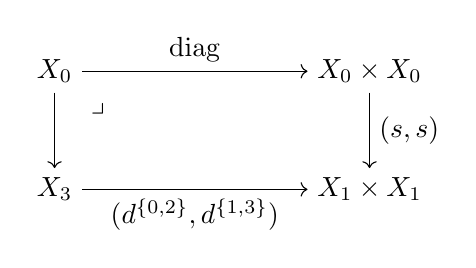
\begin{tikzpicture}[auto,->] 
    \node (tl) at (0,1.5) {$X_0$}; 
    \node (tr) at (4,1.5) {$X_0 \times X_0$};
    \node (bl) at (0,0) {$X_3$}; 
    \node (br) at (4,0) {$X_1 \times X_1$}; 
    % horizontal lines
    \draw (tl) -- node {$\mathrm{diag}$} (tr); 
    \draw (bl) -- node[swap] {$(d^{\{0,2\}},d^{\{1,3\}})$} (br); 
    % vertical lines
    \draw (tl) -- node[swap] {} (bl);
    \draw (tr) -- node {$(s,s)$} (br); 
    % pullback symbol (\lrcorner) in the lower right corner of (tl)
    \node at ([xshift=0.2cm, yshift=-0.2cm] tl.south east) {$\lrcorner$};
  \end{tikzpicture}\]
\end{definition}

The completeness condition can be understood as indicating that the higher simplices of a complete Segal simplicial anima correspond to equivalences related to its degenerate edges.

\begin{proposition}
  The Rezk nerve $\N^r : \Cat \to \Fun(\N(\Delta)^{\myop},\An)$ is fully faithful.
  Moreover, its essential image precisely consists of complete Segal simplicial anima.
\end{proposition}

\subsection{The algebraic K-Theory}

\begin{definition}
  Let $\C$ be a category with finite limits.
  For every $n \geq 0$, we let $Q_{n}(\C)$ denote the full subcategory of $\Fun(\TwArr[n],\C)$ spanned by the diagrams which take every square in $\TwArr[n]$ to a Cartesian square in $\C$.

  The construction $n \mapsto Q_{n}(\C)$ determines a functor 
  \begin{align*}
    Q(\C) : \N(\Delta)^{\myop} \to \Catlex
  \end{align*}
  and furthermore, the construction $\C \mapsto Q(\C)$ defines a functor 
  \begin{align*}
    Q : \Catlex \to \Fun(\N(\Delta)^{\myop},\Catlex).
  \end{align*}
  We will refer to this functor as the \textit{(Quillen's) Q-construction}.
\end{definition}

\begin{proposition}
  Let $\C$ be a category with finite limits.
  Then the simplicial object in $\Catlex$
  \begin{align*}
    Q(\C) : \N(\Delta)^{\myop} \to \Catlex
  \end{align*}
  is complete Segal.
  In particular, the simplicial anima 
  \begin{align*}
    \core Q(\C) : \N(\Delta)^{\myop} \to \An
  \end{align*}
  is complete Segal.
\end{proposition}

This proposition follows from the following lemmata.

\begin{notation}
  For every $n \geq 0$, we let $\J_n$ denote the full subcategory of $\TwArr[n]$ spanned by the images of objects $(i \leq j)$ in $[n]$ satisfying $j \leq i+1$.
\end{notation}

\begin{lemma}
  Let $\C$ be a category with finite limits, and let $F : \TwArr[n] \to \E$ be a functor.
  The following conditions are equivalent:
  \begin{enumerate}
    \item The functor $F$ belongs to $Q_n(\C)$.
    \item The functor $F$ is a right Kan extension of its restriction to $\J_n$ along the inclusion $\J_n \subseteq \TwArr[n]$.
  \end{enumerate}
\end{lemma}

\begin{lemma} \label{lem.Q_nC_is_equivalent_to_FunJ_n_C}
  Let $\C$ be a category with finite limits.
  Then the restriction of $\Fun(\TwArr[n],\C)$ along the inclusion $\J_n \subseteq \TwArr[n]$ induces an equivalence of categories
  \begin{align*}
    Q_n(\C) \to \Fun(\J_n,\C).
  \end{align*} 
\end{lemma}

\begin{remark}
  \Cref{lem.Q_nC_is_equivalent_to_FunJ_n_C} implies that, if $\C$ is stable, then $Q_n(\C)$ is stable.
  Therefore we obtain functors
  \begin{align*}
    Q(\C) : \N(\Delta)^{\myop} \to \Catst ~~ \text{and} ~~ Q : \Catst \to \Fun(\N(\Delta)^{\myop},\Catst).
  \end{align*}
  Moreover, for every stable category $\C$, the category $Q_n(\C)$ is a complete Segal simplicial anima, since $\Catst$ is stable under finite limits in $\Cat$.
\end{remark}

\begin{definition}
  Let $\C$ be a category with finite limits.
  Then we define the \textit{category of spans} in $\C$ as 
  \begin{align*}
    \Span(\C) := \asscat \core Q(\C).
  \end{align*}

  The construction $\C \mapsto \Span(\C)$ determines a functor 
  \begin{align*}
    \Span : \Catlex \to \Cat.
  \end{align*}
\end{definition}

\begin{definition} \label{def.algebraic_k-anima_using_Q}
  Let $\C$ be a stable category.
  Then we define the \textit{algebraic K-anima} (or \textit{algebraic K-theory anima}, or \textit{projective class anima}) as 
  \begin{align*}
    \K(\C) := \Omega|\Span(\C)| \simeq \Omega|\core Q(\C)|
  \end{align*}
  where the base object of the loop space is given by the zero object of $\Span(\C)$.

  The construction $\C \mapsto \K(\C)$ determines a functor 
  \begin{align*}
    \K : \Catst \to \An. 
  \end{align*}
  We will refer to this functor as the \textit{algebraic K-theory} (or \textit{algebraic K-functor}).
\end{definition}

\begin{definition}
  Let $\C$ be a stable category.
  For every $n \geq 1$, we define the \textit{$n$-th K-group} of $\C$ as the abelian group 
  \begin{align*}
    \K_n(\C) := \pi_n\K(\C).
  \end{align*}
\end{definition}

\begin{remark}
  Let $\C$ be a stable category.
  Then we have an equivalence 
  \begin{align*}
    \pi_0\K(\C) \simeq \K_0(\C)
  \end{align*}
  where $\K_0(\C)$ is the Grothendieck group of $\C$.
\end{remark}

\subsection{Waldhausen's S-Construction}

In this section, we construct the algebraic K-theory using Waldhausen's S-construction. 

\begin{definition}
  Let $\C$ be a stable category.
  An \textit{$[n]$-gapped object} of $\C$ is a functor $F : \Ar[n] \to \C$ which satisfies the following properties:
  \begin{enumerate}
    \item For every $0 \leq i \leq n$, $F(i,i)$ is a zero object of $\C$.
    \item For every $i \leq j \leq k$, the following diagram is a (co)Cartesian diagram in $\C$.
    \[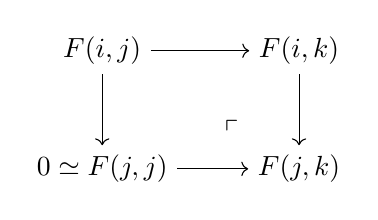
\begin{tikzpicture}[auto,->] 
      \node (tl) at (0,1.5) {$F(i,j)$}; 
      \node (tr) at (2.5,1.5) {$F(i,k)$};
      \node (bl) at (0,0) {$0 \simeq F(j,j)$}; 
      \node (br) at (2.5,0) {$F(j,k)$}; 
      % horizontal lines
      \draw (tl) -- node {} (tr); 
      \draw (bl) -- node[swap] {} (br); 
      % vertical lines
      \draw (tl) -- node[swap] {} (bl);
      \draw (tr) -- node {} (br); 
      % pushout symbol (\ulcorner) in the upper left corner of (br)
      \node at ([xshift=-1.5cm, yshift=0.8cm] br.south east) {$\ulcorner$};
    \end{tikzpicture}\]
  \end{enumerate}
  We let $S_n(\C)$ denote the full subcategory of $\Fun(\Ar[n],\C)$ spanned by the $[n]$-gapped objects of $\C$.
\end{definition}

\begin{remark}
  Let $\C$ be a stable category.
  We can describe the low-dimensional simplices of $S_n(\C)$.
  \begin{itemize}
    \item The category $S_0(\C)$ is the full subcategory of $\C$ spanned by the zero objects of $\C$. 
    Thus $S_0(\C)$ is contractible.
    \item The category $S_1(\C)$ is equivalent to $\C$, since every object of $S_1(\C)$ is of the form $0 \to X \to 0$, where $X$ is an object of $\C$.
    \item The category $S_2(\C)$ is equivalent to the arrow category $\Ar(\C)$ of $\C$, since every object of $S_2(\C)$ is of the form $0 \to X' \to X \to X'' \to 0$, where $X' \to X \to X''$ is a cofiber sequence in $\C$. 
  \end{itemize}
\end{remark}

\begin{remark}
  Let $\C$ be a stable category.
  We have an equivalence of categories 
  \begin{align*}
    S_n(\C) \simeq \Fun([n-1],\C)
  \end{align*}
  for every $n \geq 0$.
  Thus, if $\C$ is stable, then $S_n(\C)$ is stable.
\end{remark}

\begin{definition}
  The construction $n \mapsto S_n(\C)$ determines a functor 
  \begin{align*}
    S(\C) : \N(\Delta)^{\myop} \to \Catst
  \end{align*}
  and furthermore, the construction $\C \mapsto S(\C)$ determines a functor 
  \begin{align*}
    S : \Catst \to \Fun(\N(\Delta)^{\myop},\Catst).
  \end{align*}
  We will refer to this functor as \textit{(Waldhausen's) S-construction}.
\end{definition}

\begin{definition} \label{def.algebraic_k-anima_using_S}
  Let $\C$ be a stable category.
  Then we define the \textit{algebraic K-anima} as 
  \begin{align*}
    \K_S(\C) := \Omega|\core S(\C)|.
  \end{align*}

  The construction $\C \mapsto \K_S(\C)$ determines a functor 
  \begin{align*}
    \K_S : \Catst \to \An.
  \end{align*}
  We will refer to this functor as the \textit{algebraic K-theory}.
\end{definition}
 
\begin{remark} % p82
  Let $\C$ be a stable category.
  Then the anima $|\core S(\C)|$ admits a canonical base point given by a map 
  \begin{align*}
    0 \simeq \core S_0(\C) \to |\core S(\C)|.
  \end{align*}
  Moreover, $|\core S(\C)|$ is connected, since the canonical map 
  \begin{align*}
    0 \simeq \pi_0 \core S_0(\C) \to \pi_0 |\core S(\C)|
  \end{align*}
  is surjective.
\end{remark}

\begin{proposition}
  The two definitions of algebraic K-anima (\cref{def.algebraic_k-anima_using_Q,def.algebraic_k-anima_using_S}) induce an equivalence of anima
  \begin{align*}
    \K(\C) \simeq \K_S(\C)
  \end{align*}
  for every stable category $\C$.
\end{proposition}


\section{The Additivity Theorem}

\subsection{The Additivity Theorem}

The goal of this section is to prove the additivity theorem.

\begin{theorem}[\cite{HLS23} Theorem.4.1 (The Additivity Theorem)] \label{thrm.additivity_theorem}
  Let $\C$ be a stable category.
  Then the source-target projection induces an equivalence of anima 
  \begin{align*}
    (s,t) : |\Span(\Ar(\C))| \to |\Span(\C)|^2.
  \end{align*}
\end{theorem}

The proof of \cref{thrm.additivity_theorem} follows from the next two propositions.

\begin{proposition}
  Let $\C$ be a stable category.
  Then there are canonical equivalences of categories
  \begin{align*}
    \Span(\C) \to \Span(\C^{\myop}) \quad \text{and} \quad \Span(\Ar(\C)) \simeq \Span(\TwArr(\C)).
  \end{align*}
  Moreover, they fit together into a natural commutative diagram 
  \[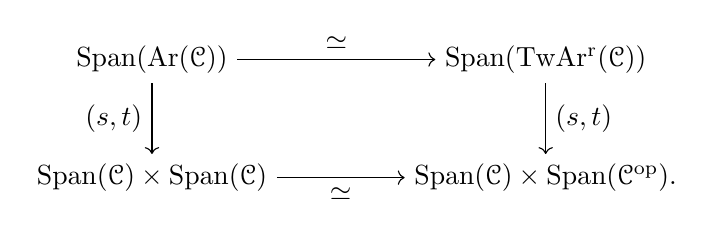
\begin{tikzpicture}[auto,->] 
    \node (tl) at (0,1.5) {$\Span(\Ar(\C))$}; 
    \node (tr) at (5,1.5) {$\Span(\TwArr(\C))$};
    \node (bl) at (0,0) {$\Span(\C) \times \Span(\C)$}; 
    \node (br) at (5,0) {$\Span(\C) \times \Span(\C^{\myop}).$}; 
    \draw (tl) -- node {$\simeq$} (tr); 
    \draw (bl) -- node[swap] {$\simeq$} (br); 
    \draw (tl) -- node[swap] {$(s,t)$} (bl);
    \draw (tr) -- node {$(s,t)$} (br); 
  \end{tikzpicture}\]
\end{proposition}

\begin{proposition}
  Let $\C$ be a stable category.
  Then the source-target projection 
  \begin{align*}
    (s,t) : \Span(\TwArr(\C)) \to \Span(\C) \times \Span(\C^{\myop})
  \end{align*}
  is cofinal.
\end{proposition}

We introduce some corollaries of the additivity theorem.

\begin{corollary}
  Let $\C$ be a stable category.
  Then the source-target projection $(s,t) : \Ar(\C) \to \C $ induces an equivalence of anima
  \begin{align*}
    \K(\Ar(\C)) \to \K(\C)^2.
  \end{align*}
\end{corollary}

\begin{corollary} \label{cor.algebraic_k-theory_is_additive_grouplike}
  The algebraic K-theory $\K : \Catst \to \An$ is additive grouplike.
\end{corollary}

\begin{proposition}[Eilenberg swindle]
  Let $\C$ be a stable category with countable coproducts.
  For every additive grouplike functor $F : \Catst \to \An$, we have 
  \begin{align*}
    F(\C) \simeq 0
  \end{align*}
  for every stable category $\C$.
  In particular, $i$-th K-groups vanish for every $i \geq 0$.
\end{proposition}

\subsection{The algebraic K-Theory Spectrum}

We can define an algebraic K-theory spectrum $\K_{\geq 0} : \Catst \to \Sp$.

\begin{definition}
  \Cref{cor.algebraic_k-theory_is_additive_grouplike} implies that the K-theory functor lifts to a functor 
  \begin{align*}
    \K : \Catst \to \Grp(\An).
  \end{align*}
  Since we have the equivalence $\Grp(\An) \simeq \Sp_{\geq 0}$, we obtain a functor 
  \begin{align*}
    \K_{\geq 0} : \Catst \to \Sp_{\geq 0} \subseteq \Sp.
  \end{align*}
  We will refer to this functor as the \textit{algebraic K-theory spectrum}.
\end{definition}

\begin{remark}
  There is the equivalence $\Omega^\infty : \Sp_{\geq 0} \rightleftarrows \Grp(\An) : \Sigma^\infty$.
  We can recover the algebraic K-functor from algebraic K-theory spectrum as 
  \begin{align*}
    \K \simeq \Omega^\infty \K_{\geq 0} :  \Catst \to \Sp_{\geq 0} \simeq \Grp(\An) 
  \end{align*}
  since $\Sigma^\infty$ is fully faithful.
\end{remark}


\section{The Universality Theorem}

The goal of this section is to prove the universality theorem.

\begin{theorem}[\cite{HLS23} Theorem.5.1 (The Universality Theorem)] \label{thrm.universality_theorem}
  The algebraic K-theory $\K : \Catst \to \An$ is an initial additive grouplike functor under the core functor $\core : \Catst \to \An$.
  That is, the natural map $\tau : \core \Rightarrow \K$ is an initial object in the category $\Fun(\Catst,\An)^{\mathrm{add,grp}}_{\core/}$.
\end{theorem}

\begin{notation}
  Let $F : \Catst \to \An$ be a reduced functor.
  We denote a functor 
  \begin{align*}
    GF(-) := \Omega|FQ(-)| : \Catst \to \An. 
  \end{align*}
  For example, the functor $G\core$ is equivalent to the algebraic K-theory $\K$.
\end{notation}

\begin{proof}
  We want to show that the natural transformation $\tau : \core \Rightarrow \K$ induces an equivalence
  \begin{align*}
    \tau^{\ast} : \Nat(\K,F) \to \Nat(\core,F)
  \end{align*}
  for every additive grouplike functor $F : \Catst \to \An$.
  
  Now consider the following diagram 
  \[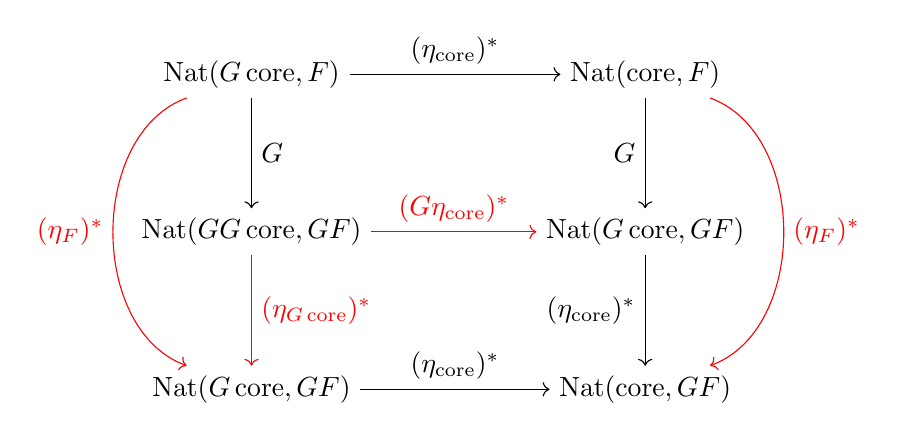
\begin{tikzpicture}[auto,->]
    \node (tl) at (0,4) {$\Nat(G\core,F)$};
    \node (tr) at (5,4) {$\Nat(\core,F)$};
    \node (ml) at (0,2) {$\Nat(GG\core,GF)$};
    \node (mr) at (5,2) {$\Nat(G\core,GF)$};
    \node (bl) at (0,0) {$\Nat(G\core,GF)$};
    \node (br) at (5,0) {$\Nat(\core,GF)$};
    % horizontal lines
    \draw (tl) -- node {$(\eta_{\core})^\ast$} (tr);
    \draw[red] (ml) -- node {$(G\eta_{\core})^\ast$} (mr);
    \draw (bl) -- node {$(\eta_{\core})^\ast$} (br);
    % vertical lines
    \draw (tl) -- node {$G$} (ml);
    \draw[red] (ml) -- node {$(\eta_{G\core})^\ast$} (bl);
    \draw (tr) -- node[swap] {$G$} (mr);
    \draw (mr) -- node[swap] {$(\eta_{\core})^\ast$} (br); 
    % bending lines 
    \draw[bend right=70,red] (tl) to node[swap] {$(\eta_{F})^\ast$} (bl);
    \draw[bend left=70,red] (tr) to node {$(\eta_{F})^\ast$} (br);
  \end{tikzpicture}\]
  where the upper square commutes since $G$ is a functor, and the other there parts commute since $\eta$ is natural.
  Suppose the red-colored maps are equivalent, then we can show that the upper horizontal map $(\eta_{\core})^\ast$ is an equivalence.
  If we apply this to the case $F \simeq \core$, then we obtain the desired result.
  This assumption follows from the next two propositions.
\end{proof}

The next proposition implies that $(\eta_{F})_{\ast}$ and $(G\eta_{\core})^{\ast}$ are equivalences.

\begin{proposition}
  Let $F : \Catst \to \An$ be an additive grouplike functor.
  Then the natural transformation
  \begin{align*}
    \eta_{F} : F \Rightarrow GF
  \end{align*}
  is an equivalence. 
\end{proposition}

The next proposition implies that $(\eta_{G\core})$ is an equivalence.

\begin{proposition}
  Let $F : \Catst \to \An$ be an additive functor.
  Then the two natural transformations
  \begin{align*}
    \eta_{GF} , G\eta_{F} : GF \Rightarrow GGF
  \end{align*}
  differ by an automorphism of the target.
  That is, the following diagram commutes
  \[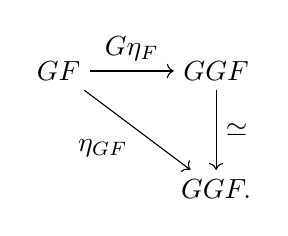
\begin{tikzpicture}[auto,->] 
    \node (tl) at (0,1.5) {$GF$}; 
    \node (tr) at (2,1.5) {$GGF$};
    \node (br) at (2,0) {$GGF.$}; 
    \draw (tl) -- node {$G\eta_{F}$} (tr); 
    \draw (tr) -- node {$\simeq$} (br); 
    \draw (tl) -- node[swap] {$\eta_{GF}$} (br);
  \end{tikzpicture}\] 
\end{proposition}


\section{The Localization Theorem}

The goal of this section is to prove the localization theorem.

\begin{theorem}[\cite{HLS23} Theorem.6.1 (The Localization Theorem)] \label{thrm.localization_theorem}
  The algebraic K-theory $\K : \Catst \to \An$ and the algebraic K-theory spectrum $\K_{\geq 0} : \Catst \to \Sp$ are Verdier-localizing.
\end{theorem}

By the corollary of \cref{thrm.Waldhausen_fibration_theorem}, an additive grouplike functor $F : \Catst \to \An$ is Verdier-localizing if and only if it satisfies the following condition:
\begin{itemize}
  \item[$(\ast)$] For every Verdier sequence $\C \to \D \to \E$, the canonical map $|F\Fun^{\C}([-],\D)| \to F(\E)$ is an equivalence of anima.
\end{itemize}

The next proposition implies that it is enough to prove that the core functor satisfies $(\ast)$.

\begin{proposition}
  Let $F : \Catst \to \An$ be an additive functor.
  If $F$ satisfies $(\ast)$, then $|FQ(-)|$ and $\Omega|FQ(-)|$ also satisfy $(\ast)$.
\end{proposition}

\begin{remark}
  If the core functor satisfies $(\ast)$, then the K-theory functor also satisfies $(\ast)$.
  Indeed, we can write 
  \begin{align*}
    \K(-) 
    \simeq \Omega|\Span(-)| 
    \simeq \Omega|\asscat\core Q(-)| 
    \simeq \Omega|\core Q(-)|.
  \end{align*}
\end{remark}

To prove the proposition, we need the following lemma.

\begin{lemma}
  Verdier sequences are stable under applying the functor 
  \begin{align*}
    \Fun(\I,-) : \Catst \to \Catst
  \end{align*}
  for every finite poset $\I$.
\end{lemma}

From the above discussion, we need to show that the core functor satisfies $(\ast)$.
Let $\D$ be a stable category, and let $\C$ be a stable subcategory of $\D$.
We let $\D_{\C}$ denote the full subcategory of $\D$ spanned by the equivalences modulo $\C$ in $\D$.
Then we obtain 
\begin{align*}
  \core\Fun^{\C}([-],\D) 
  \simeq \core\Fun([-],\D_{\C})
  \simeq \Map_{\Cat}([-],\D_{\C})
  \simeq \N^r(\D_{\C}).
\end{align*}
Since the canonical map $|\N^r(\D_{\C})| \to |\D_{\C}|$ is an equivalence of anima, we have an equivalence 
\begin{align*}
  |\core\Fun^{\C}([-],\D)| \simeq |\D_{\C}|.
\end{align*}
Thus it suffices to show the following proposition.

\begin{proposition}
  Let $\D$ be a stable category, and let $\C$ be a stable subcategory of $\D$.
  We let $\D_{\C}$ denote the full subcategory of $\D$ spanned by the equivalences modulo $\C$ in $\D$.
  Then the map 
  \begin{align*}
    |\D_{\C}| \to \core(\D/\C)
  \end{align*}
  is faithful.
  If the inclusion $\C \subseteq \D$ is a Verdier inclusion, then this map is an equivalence.
\end{proposition}

This proposition is a special case of the following proposition.

\begin{proposition}
  Let $\C$ be a category, and let $S$ be a subcategory of $\C$.
  If $S$ is closed under 2-out-of-3 and pushouts in $\C$, then a map 
  \begin{align*}
    |S| = S[S^{-1}] \to \C
  \end{align*}
  is faithful. 
  Moreover, the following conditions are equivalent:
  \begin{enumerate}
    \item The inclusion $|S| \subseteq \core\C[S^{-1}]$ is fully faithful.
    \item The category $S$ is closed under 2-out-of-6 in $\C$.
    \item A morphism in $\D$ belongs to $S$ if and only if its source and target are in $S$ and it is invertible in $\C[S^{-1}]$.
  \end{enumerate}
\end{proposition}


\section{The Cofinality Theorem}

The goal of this section is to prove the cofinality theorem.

\begin{theorem}[\cite{HLS23} Theorem.7.1 (The Cofinality Theorem)] \label{thrm.cofinality_theorem}
  Let $f : \C \to \D$ be a functor between stable categories.
  If $f$ is a dense inclusion, then it induces a fiber sequence
  \begin{align*}
    \K(\C) \to \K(\D) \to \K_0(\D)/\K_0(\C).
  \end{align*}
  In particular, maps of abelian groups
  \begin{align*}
    \K_i(\C) \to \K_i(\D)
  \end{align*}
  are isomorphisms for every $i \geq 1$, and there exists a short exact sequence 
  \begin{align*}
    0 \to \K_0(\C) \to \K_0(\D) \to \K_0(\D)/\K_0(\C) \to 0.
  \end{align*}
\end{theorem}

\begin{definition}
  Let $f : X \to Y$ be a map of $\Einf$-monoids in $\An$.
  We will say that $f$ is \textit{cofinal} if it satisfies the following conditions:
  \begin{enumerate}
    \item The map $\pi_0(f) : \pi_0(X) \to \pi_0(Y)$ is an inclusion.
    \item For every object $y$ in $\pi_0(Y)$, there exists an object $y'$ in $\pi_0(Y)$ such that $y+y'$ in $\pi_0(X)$.
  \end{enumerate}
  We will say that a cofinal map is \textit{dense} if it satisfies the following conditions:
  \begin{enumerate}[resume]
    \setcounter{enumi}{2}
    \item An object $y$ in $\pi_0(Y)$ belongs to $\pi_0(X)$ if there exists an object $x$ in $\pi_0(X)$ such that $x+y$ in $\pi_0(X)$.
  \end{enumerate}
\end{definition}

\begin{definition}
  Let $F : \Catst \to \An$ be an additive functor.
  We will say that $F$ is \textit{Karoubian} if it satisfies the following conditions:
  \begin{enumerate}
    \item The functor $F$ takes every dense inclusion between stable categories to a dense map of $\Einf$-monoids.
    \item The functor $F$ preserves every Cartesian square in $\Catst$ whose vertical maps are dense.
  \end{enumerate}
\end{definition}

\begin{example}
  The core functor $\core : \Catst \to \An$ is Karoubian.
\end{example}

\Cref{thrm.cofinality_theorem} holds for a broader class of additive Karoubian functors.

\begin{notation}
  Let $F : \Catst \to \An$ be an additive Karoubian functor.
  We will refer to the functor
  \begin{align*}
    F^{\grp} := \Omega|FQ-|
  \end{align*}
  as the \textit{group completion} of $F$.
  For example, the functor $(\core)^{\grp}$ is equivalent to the algebraic K-theory $\K$.
\end{notation}

\begin{theorem}
  Let $F : \Catst \to \An$ be an additive Karoubian functor.
  For every dense inclusion $\C \subseteq \D$ between stable categories, the canonical map of $\Einf$-monoids
  \begin{align*}
    F(\D)/F(\C) \to F^{\grp}(\D)/F^{\grp}(\C)
  \end{align*}
  is an equivalence.
  Hence maps of abelian groups
  \begin{align*}
    \pi_iF^{\grp}(\C) \to \pi_iF^{\grp}(\D)
  \end{align*}
  are isomorphisms for every $i \geq 1$, and there exists a short exact sequence 
  \begin{align*}
    0 \to \pi_0F^{\grp}(\C) \to \pi_0F^{\grp}(\D) \to \pi_0F^{\grp}(\D)/\pi_0F^{\grp}(\C) \to 0.
  \end{align*}
\end{theorem}

\begin{corollary}
  If a functor $F : \Catst \to \An$ is additive Karoubian, then so is the group completion $F^{\grp}$ of $F$.
\end{corollary}

\begin{corollary} \label{cor.group_completion_is_Karaubi_localizing}
  Let $F : \Catst \to \An$ be an additive Karoubian functor.
  If the functor $F^{\grp}$ is Verdier-localizing, then the functor
  \begin{align*}
    F^{\grp} \circ (-)^{\natural} : \Catst \to \An
  \end{align*}
  is Karoubi-localizing.
  In particular, the functor $\K \circ (-)^{\natural} : \Catst \to \An$ is Karoubi-localizing.
\end{corollary}

\begin{corollary}
  Let $\D$ be a stable category, and let $\C$ be a dense stable subcategory of $\D$.
  Then the canonical maps of abelian groups
  \begin{align*}
    \K_i(\C) \to \K_i(\D)
  \end{align*}
  are isomorphisms for every $i \geq 1$.
\end{corollary}

\printbibliography


\end{document}